\chapter{Spark-SIFT系统的三种性能优化方案}
在上一章节中,本文介绍了整个大规模特征提取系统Spark-SIFT的设计和实现,本章节主要针对Spark-SIFT 进行性能优化。第一,针对Spark-SIFT系统加载大量小图片时,频繁的磁盘IO,读写开销较大问题作出了优化,在该问题的优化上,本文设计了一种新的数据结构来描述图片,以Key-Value的方式表示一张图片,将图片转成单条记录的形式,然后将众多的记录合并并且序列化保存供后续操作使用,以提高读写效率;第二,由于Spark的任务划分及分配机制,导致Spark-SIFT系统在处理图片大小差异很大的数据集,会出现负载不均衡的现象,本文提出了分割式特征提取算法以解决处理过程中出现的负载不均衡问题;第三,因为分割式特征提取算法会引用shuffle操作,当处理的图片量很大时,会严重影响系统的性能,因此本文在分割式特征提取算法的基础上改进,提出了shuffle-efficient的特征提取算法,以解决shuffle操作带来的性能问题。

\section{key-value的图片描述数据结构}
因为图片和图片间是分立的,整个数据集是一个个分立的文件组成,spark在加载的时候也只能是一个个加载,如果每个文件很小,文件的数量有多,这情况下读写的效率是很低的。那么怎样才能提高加载时候的性能呢?在spark下处理文本信息会比较多,在处理文本信息时,spark是把一整个文本文件加载进来,然后每一行就是一个基本的并行单元,所以能不能把一张图片看成文本文件中的一行记录,然后很多行记录组成一个大文本,就相当很多个图片合并在一个大文件中,那么一次性就可以加载很多图片。

在spark在处理文本文件方式的启发下,我们采用了Key-Value的方式来描述一张图片,Key就是图片的文件名,Value就是图片内容的字节流,通过这种方式,就可以用一条记录的形式描述了一张图片,然后将这些记录序列化保存到指定的hdfs目录下,在序列化方式上,Spark-SIFT选用了Hadoop的原生序列化方式,而没有采用Java序列化。这是因为Java序列化后产生的内容容量太大,分布式环境中传输时会十分占用带宽,而hadoop 序列化产生的内容十分简洁,容量更小,这有助于减少分布式处理时的数据传输量。通过这种将图片转换成记录的形式,Spark在读取该目录时,就可以一次性将目录下的记录加载进来,从能提供了读写的效率。图\ref{fig:kv_image}显示了整个设计的框架。
\begin{figure}[htp]
\centering
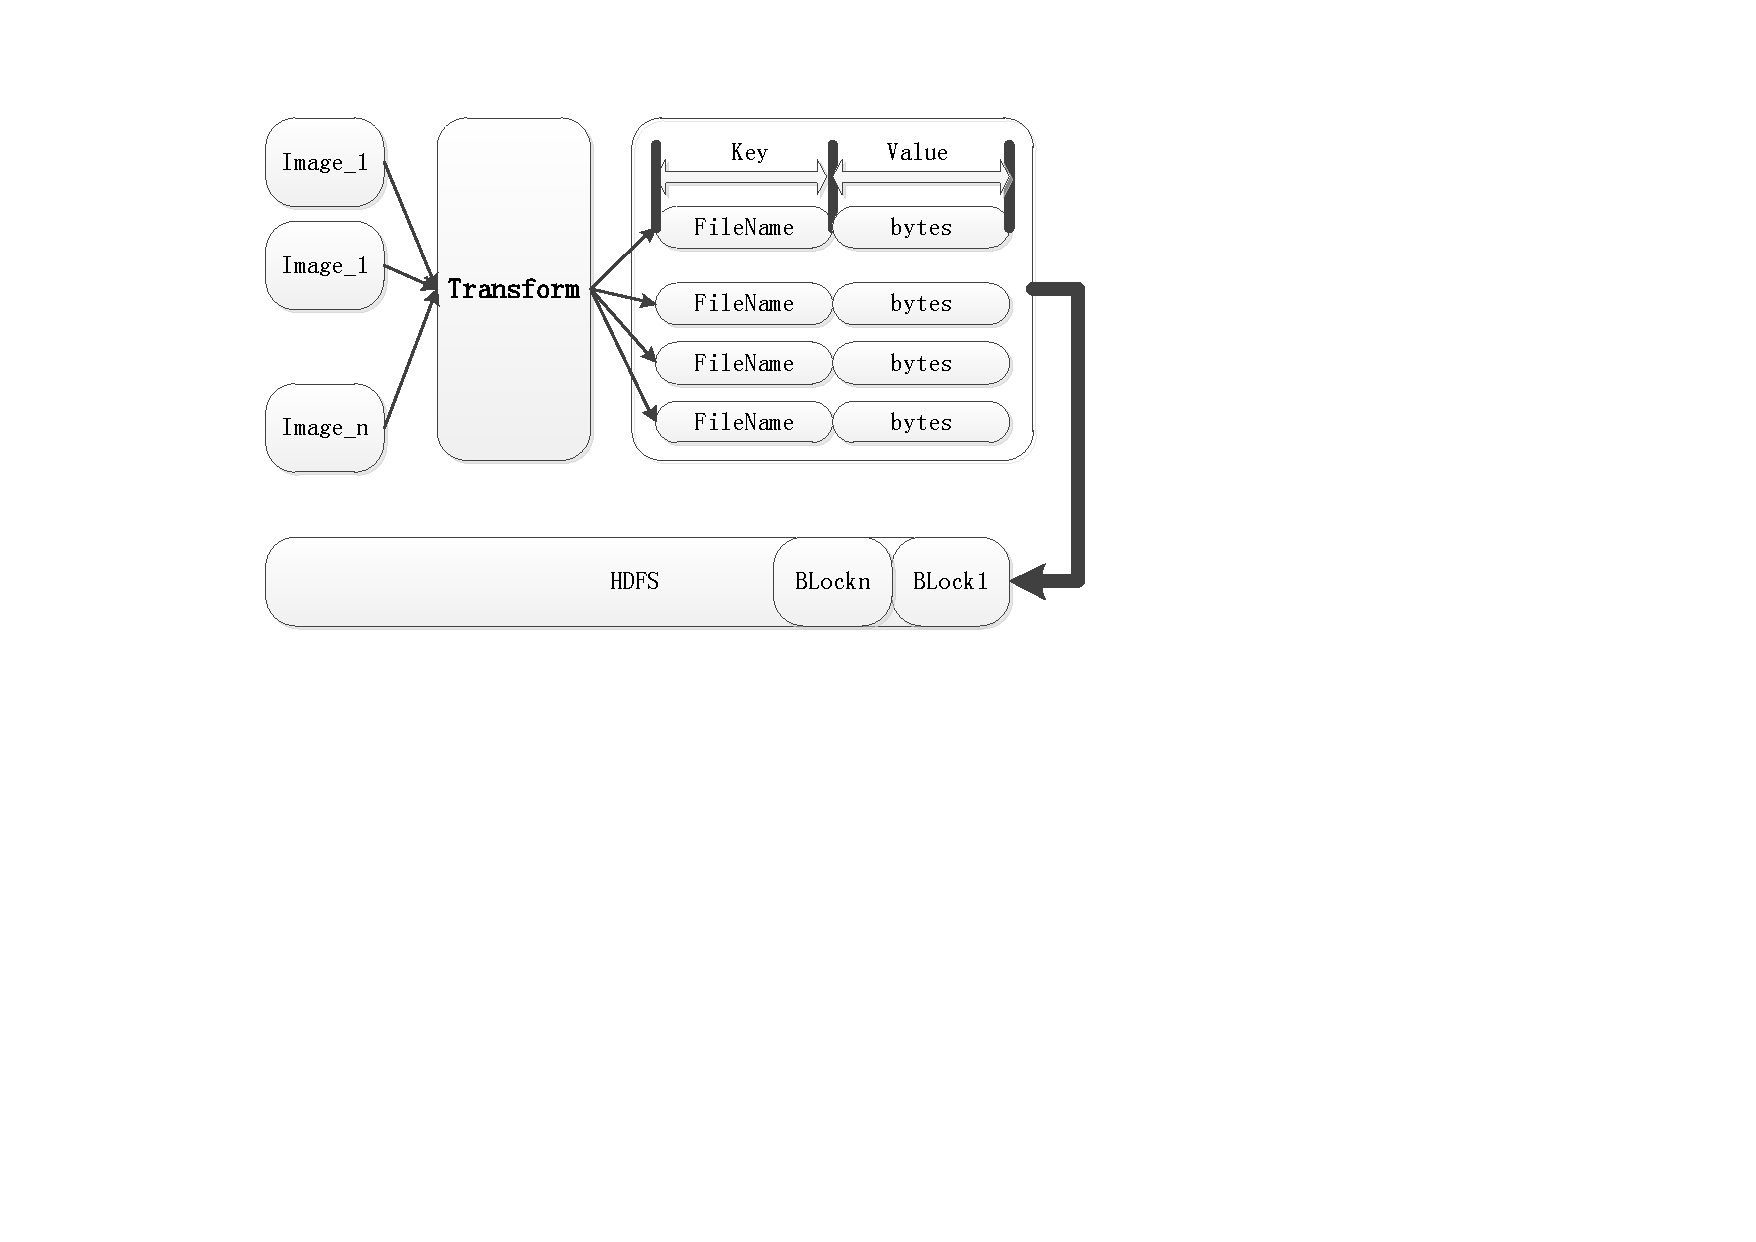
\includegraphics{kv_image}
\caption{key-value描述图片方式}
\label{fig:kv_image}
\end{figure}

具体的实验数据将会在第五章中给出,在此先不进行数据的分析。
\section{分割式图片特征提取算法}
Spark-SIFT在对某些数据集进行特征提取时会出现严重的负载不均衡现象。以提取200MB图片集合的特征为例,集合中图片的大小为2MB或4MB,但其处理时间有时会比处理一个1GB 的图片集合(图片大小在100到200KB 之间)还要长。观察Spark的Executors监控页面我们发现,200MB图片集处理时间较长往往是因为某个Executor的执行速度特别慢,而此时其他Executors都已经完成了分配的任务,处于空闲状态。

有两个原因引发了Spark-SIFT系统在处理图片差异较大数据集时出现的负载不平衡现象。首先与SIFT算法自身的特点有关,SIFT算法的时间复杂度和图片大小相关,为$O(N^5)$,并且SIFT算法的空间复杂度也十分大,另外Spark本身也是很耗内存,这样就导致运行过程中很耗内存,当内存占用过高时,CPU的利用率无法上去,这样就导致运算速度十分慢;其次是Spark任务分配机制,Spark任务分配按照大小区分,划分时仅考虑了各个任务所处理的图片总容量,而忽略了任务中图片大小的因素。那么,如果图片的大小不一样,一个任务都是大图片,而另外一个是小图片,那么大图片的运行时间会更长,但是Spark分配机制认为只要两个任务是size 一样,那么两个任务运行时间基本一样。同时Spark分配到Executor 上的任务,在没有失败的情况下,是不会回收的,尽管有其他空闲的Executor,这样就会出现其他Executors都是空闲的,而只有一个Executor在运算的情况。

针对上面的问题,我们采用分割图片的方式,使图片集中各图片的大小尽可能相同,以适应Spark的任务分配和负载均衡策略,使各个任务的运行时间基本相同。图片分割的具体工作原理如图\ref{fig:segmentation}所示:
\begin{figure}[htp]
\centering
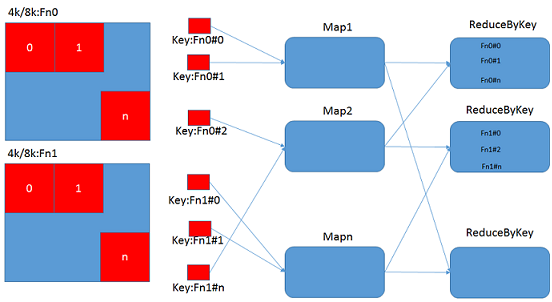
\includegraphics[width=130mm,height=93mm]{segmentation}
\caption{分割式特征提取算法}
\label{fig:segmentation}
\end{figure}

本文将分割后得到的图片大小称为分割大小,它会影响特征提取的速度和结果的精度。理论上,分割后的图片越小,每张图片的处理速度越快,但是由于子图之间会产生边缘噪声,导致提取出的特征点存在较大的误差。通过实验,我们选择500×500作为基本分割大小,它既可以保证特征提取的速度足够快,又可以使得结果误差比较小,第五章将详细介绍测试结果和选择依据。

算法流程如图\ref{fig:alg_segmentation}所示,在map任务1,我们将一张图片按照设置的模板大小进行划分,划分为多个子块,每个子块由图片文件名加模块下标,模块的长,模块的宽以及模块的像素内容字节数组四个元素组成。因为在map任务1结束后,一张图片的子块只是位于一个独立的数组中,数组和数组间是分立的,这样并行操作只能在单个数组里面进行,这种情况并行化程度是不高的,因此在map任务1结束后,我们又启用了一个flatMap算子,通过flatMap操作,我们将数组扁平化,将每个数组的元素抽取出来,组成一个大的数组,使得并行化操作在所有图片的子块中执行,这样就可以大大提高并行化程度。当图片子块被扁平化之后,我们又重构了子块的表示方式,在map 任务1中,子块的表示方式是(fname,row,col,bytes),在map任务2 中,以(fname,(row,col,bytes))的方式表示一个子块,这样子块就可以表示为key-value的形式了,这种表示方式也为后面处理完子块后收集同一张图片的子块提供了方便;在map任务3中,进行子块图片的特征提取工作,在这个任务中,我们还进行key的重构工作,因为之前子块的key是带有下标的,但是在特征提取完之后就不需要带有下标了,因此我们将子块图片的下标去掉,那么同一张图片的子块的key就是一样的,最后提取的出来的特征点集以(fnkey,kpslist.tolist)的形式表示,其中fnkey就是子块图片的所属图片的文件名,kpslist就是子块图片提取的特征点集合,kpslist.tolist表示将其转化成list的形式;在map 任务3结束后,我们启动了一个reduceByKey 的任务,在该任务中,我们按照key进行value合并,通过这个操作,同一张图片的划分为不同子块提取的特征点集就会收集到一个数组中,数组的每一个元素对应子块提取的特征点集;在最后的一个任务map任务4中,我们将提取的特征点集进行序列化,最后保存到HDFS中。
\begin{figure}[htp]
\centering
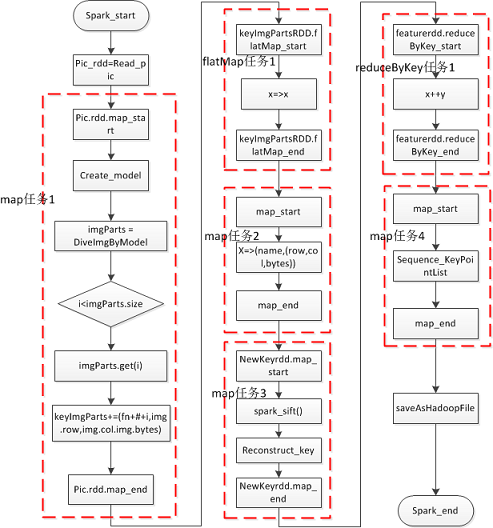
\includegraphics[width=136mm,height=152mm]{alg_segmentation}
\caption{分割式特征提取算法流程图}
\label{fig:alg_segmentation}
\end{figure}

子块划分算法如下所示:
\begin{algorithm}[htbp]
  \caption{子块划分算法}
  \label{algDiveModel}
  输入:原始图片像素数组orgin,划分模板modelImg\\
  输出:子块数组imgParts
  \begin{algorithmic}[1]
    \STATE $rowParts\leftarrow imgrow/modelImg.row$
    \STATE $colParts\leftarrow imgcol/modelImg.col$
    \FOR{$i=0$ to $rowParts$}
    \IF{$i==rowParts-1$}
        \STATE $rowOffset\leftarrow row + imgrow\%modelImg.row-1$
    \ELSE
        \STATE $rowOffset\leftarrow row - 1$
    \ENDIF
    \FOR{$j=0$ to $colParts$}
    \IF{$j==colParts-1$}
        \STATE $colOffset\leftarrow col + imgcol\%modelImg.col-1$
    \ELSE
        \STATE $colOffset\leftarrow col - 1$
    \ENDIF
    \STATE $img\leftarrow getOnePart$
    \STATE imgParts.add(img)
    \ENDFOR
    \ENDFOR
    \STATE Return imgParts
  \end{algorithmic}
\end{algorithm}

算法是利用模板进行逐行扫描思想,1,2两步获取图片被划分的块数,第3步进入一个嵌套循环,分别是按rowParts和colParts遍历,根据rowOffset和colOffset 依次得到相应的子块,获取步骤为第15步,将每次获取到的子块添加到imgParts数组中,函数结束后返回imgParts数组。 因为图片大小和模板大小不是一个整倍数的关系,所以在嵌套遍历中加入了最后一次的特殊处理,直接赋值rowOffset 和colOffset,即第5 步和第7 步。获取子块函数getOnePart关键伪代码如下所示:
\begin{lstlisting}[language=Java]
public static SequenceImage GetOnePart(byte [][]pixel, int rowStart, int colStart, int roffset, int coffset){
    byte [][]tpixel = new byte[roffset+1][coffset+1];

    //根据行偏移和列偏移获取相应区域的像素块
    for (int i = 0; i <= roffset; i++) {
        for (int j = 0; j <= coffset; j++) {
            tpixel[i][j] = pixel[i+rowStart][j+colStart];
        }
    }

    SequenceImage partimg = new SequenceImage(roffset+1,coffset+1,tpixel);

    return partimg;//返回指定像素块
}
\end{lstlisting}

至此,分割式特征提取算法介绍完毕,在第五章中,我们会给出相应的实验数据分析。
\section{Shuffle-Efficient的特征提取算法}
在上一节中,本文介绍了分割式特征提取算法,在该算法中,我们将大图片划分为子块,目的是解决Spark-SIFT系统提取过程中出现的负载不均衡问题。虽然分割式解决了处理过程中负载不均衡问题,但是该算法也引入了Shuffle操作,Shuffle操作是spark处理中十分影响性能的一个操作,因此本小节中将会针对分割式提取算法中的Shuffle操作进行优化,以进一步提高Spark-SIFT系统的处理性能。
\subsection{Shuffle原理}
Spark在执行Map-Reduce操作时,需要将处理的数据集分发到各个节点上,在数据被处理完后,再从各个节点上回收结果,这就是一个具有Shuffle操作的过程。Shuffle操作存在大量的磁盘IO和网络传输,十分损耗性能。spark中存在两种Shuffle机制,分别是Hash Based Shuffle机制和Sort Based Shuffle机制。Hash Based Shuffle,正如名字所示,该Shuffle机制是跟Hash值相关的,这个Hash值指的是key的Hash值,Spark 会根据key的Hash值算出对应的分区,这个分区其实就是下游的一个任务,然后将上游任务的结果单独的写到一个文件中,下游的任务拉取相应的结果文件,继续任务的执行,整个过程如图\ref{fig:hash_shuffle}所示。
\begin{figure}[htp]
\centering
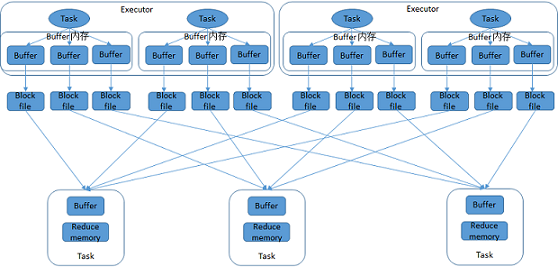
\includegraphics[width=150mm,height=59mm]{hash_shuffle}
\caption{hash based shuffle机制}
\label{fig:hash_shuffle}
\end{figure}

从Hash Based Shuffle的运行过程就可以看出,每个上游的任务都需要给下游的任务创建一个文件,过程产生文件的总数为:tasks(上游)*tasks(下游),在图\ref{fig:hash_shuffle} 中就创建了4*3个过程文件,如果上游和下游的任务数很多,那么就会有大量的中间文件被创建,而每打开一个文件都会占用内存,这将消耗大量的内存,很容易就造成内存溢出;另外读写大量的文件就会存在大量的磁盘IO操作,这也是十分损耗性能的,并且如果同一个key的结果文件散落在不同的机器的分区上,又会存在网络传输的开销。

针对Hash Based Shuffle产生大量中间文件的问题,Spark中又出现了一个Sort Based Shuffle机制,在该机制下,每个上游的任务会把结果只写到一个文件中,然后生成一个index,下游的任务根据index的信息,到对应的文件上读取上游结果信息。通过这样方式,就可以大大的减少中间文件的数量,如图\ref{fig:sort_shuffle}所示,该方式下,过程文件仅为4个。
\begin{figure}[htp]
\centering
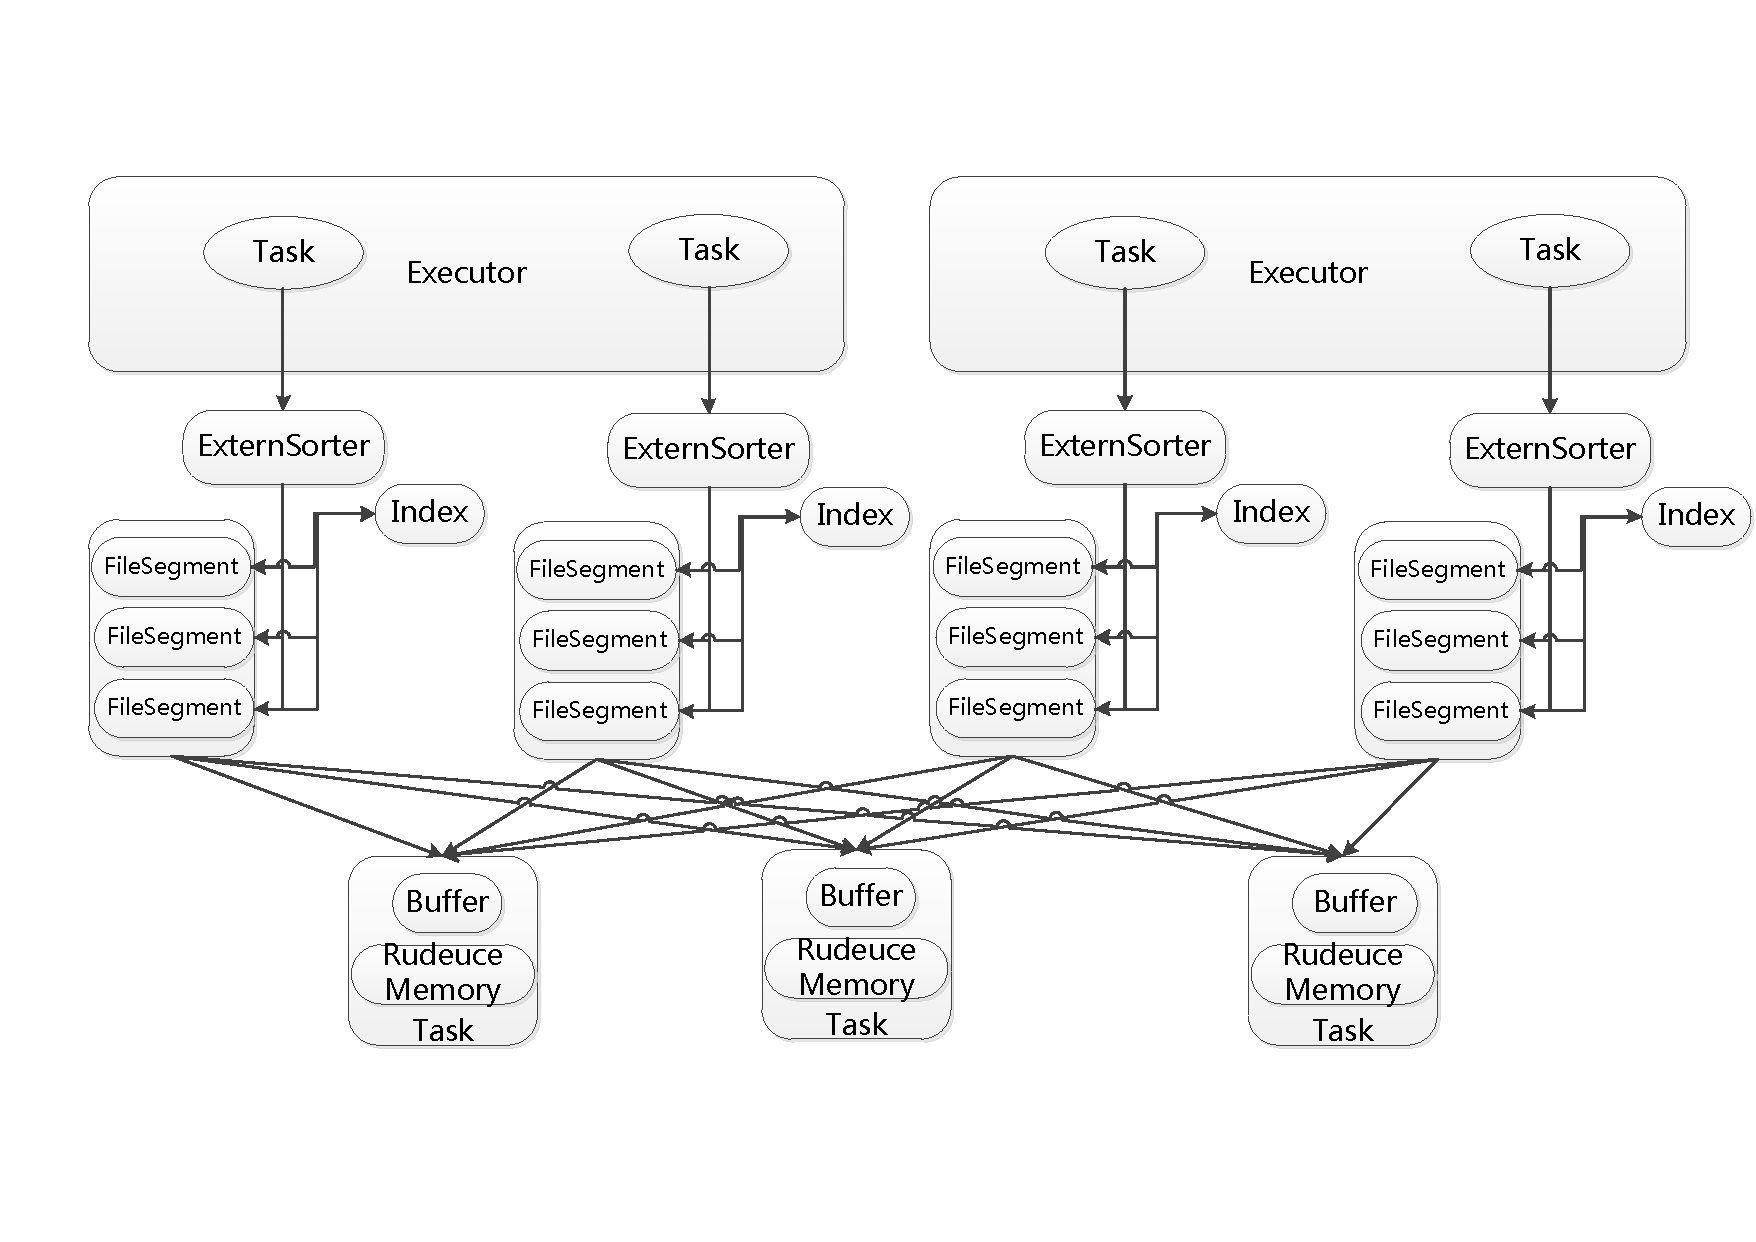
\includegraphics[width=150mm,height=59mm]{sort_shuffle}
\caption{sort based shuffle机制}
\label{fig:sort_shuffle}
\end{figure}

\subsection{高效的分区划分}
如图所示\ref{fig:seg_shuffle}在分割式算法中是存在两个Shuffle过程的,分别是将图片的子块分配到不同的分区上以及从不同的分区中收集子块特征点集,因为每张图片的子块在被收集之前,它们的key是不相等的,根据之前分割式算法分析中,它们是用图片的文件名加上子块位于图片的下标组成的。如果按照Spark的默认分区策略,Spark会按照Key的哈希值进行分区,那么同一张图片的子块就有可能会被分配到不同的分区上,也就有可能位于不同的机器上。所以当出现这样情况时,在收集同一张图片的子块时,就需要跨分区和跨机器收集,这显然会影响性能。因此本文提出了一种高效的分区策略,我们对子块进行分区时没有使用Spark 的默认分区策略,而是截取了子块key字符串的`\#`之前的字符串,然后算这个字符串的hash值,根据该hash 值对总分区数的求余值进行分区。因为同一张图片的子块它们的key字符串中`\#`字符之前的字符串是一样的,那么算出来的hash值也是一样的,所以它们的分区号也是一样的。通过这种分区方式,就可以使得同一张图片的不同子块落在同一分区上,减少了无谓的跨分区收集的网络传输开销。分区划分算法如下所示:
\begin{algorithm}[htbp]
  \caption{高效分区策略}
  \label{algDiveModel}
  输入:子块key字符串\\
  输出:子块分区号
  \begin{algorithmic}[1]
    \STATE $newKey\leftarrow key.split("\#")$
    \STATE $code\leftarrow newKey.hashCode\%numPartitions$
    \IF{$code<0$}
        \STATE $code\leftarrow code + numPartitions$
    \ENDIF
    \STATE Return code
  \end{algorithmic}
\end{algorithm}

\begin{figure}[htp]
\centering
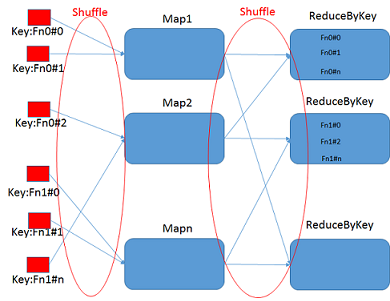
\includegraphics[width=86mm,height=95mm]{seg_shuffle}
\caption{分割式算法的Shuffle操作}
\label{fig:seg_shuffle}
\end{figure}

\section{本章小结}
本章主要介绍了针对Spark-SIFT系统的三种优化策略。首先是针对大量小文件在spark中加载低效问题,本文设计了一种用key-vaule表示图片的数据结构,将一张图片转化成一条记录,然后将多条记录合并保存,从而提高了Spark加载处理图片的效率;其次,本文针对Spark-SIFT 系统在处理图片大小差异较大的数据集时出现的负载不均衡问题,本文提出了分割式特征提取算法,将大图片划分为子块,解决了Spark-SIFT系统的负载不均衡问题同时也提高了系统的并行度;最后,本文针对分割式特征提取算法中引入的Shuffle开销,提出了Shuffle-Efficient的特征提取算法,使用了高效的分区策略,降低了Shuffle的网络开销。
